\DiaryEntry{Inside Interesting Integrals, Feynman's Trick (Chap 3)}{2022-03-21}{Integrals}

We consider a definite integral where (i) the limits depend on a parameter $\alpha$ and (ii) the integrand is parametrized by $\alpha$ as well,

\bee
I(\alpha) = \int_{a(\alpha)}^{b(\alpha)} f(x, \alpha) dx
\eee

Differentiating with respect to $\alpha$ yields (shown without proof here)

\begin{equation}\label{2022-03-21:eq1}
\boxed{
\frac{d I(\alpha)}{d \alpha} = \int_{a(\alpha)}^{b(\alpha)} \frac{ \partial f(x, \alpha) }{\partial \alpha } dx + f(b, \alpha) \frac{db}{d \alpha} - f(a, \alpha) \frac{da}{d \alpha}
}
\end{equation}

The first term comes from exchanging the integral (with respect to $x$) with the derivative (with respect to $\alpha$). The second and third term come from considering the integral change when the upper and lower term vary, respectively.

Let's start with a simple example with constant limits and $f(\alpha, x) = \alpha x$. We can calculate the integral directly as

\bee
I(\alpha) = \int_{a}^{b} \alpha x dx = \left. \frac{\alpha x^2}{2} \right|_a^b = \frac{\alpha (b^2 - a^2)}{2}
\eee

Taking the derivative yields

\bee
\frac{d I(\alpha)}{d \alpha} = \frac{b^2 - a^2}{2}
\eee

Let's calculate the derivative directly by using \eqref{2022-03-21:eq1} (we have used the fact that the limits are constant),

\bee
\frac{d I(\alpha)}{d \alpha} = \int_{a}^{b} \frac{ \partial f(x, \alpha) }{\partial \alpha } dx = \int_{a}^{b} \frac{ \partial \alpha x}{\partial \alpha } dx = \int_{a}^{b} x dx = \frac{b^2 - a^2}{2}
\eee

and this corresponds to the result obtained via direct calculation. \qed

Next we have a non-constant upper limit and we apply \eqref{2022-03-21:eq1},

\bee
I = \int_0^t ax dx \quad \frac{dI}{dt} = f(b,\alpha) \frac{db}{d \alpha} = at \cdot 1 = at
\eee

When the upper limit changes from $t$ to $t + \Delta t$, the area (integral value) changes by $at$. Direct evaluation yields $I = at^2/2$ and $dI/dt = at$. \qed

While these examples were certainly interesting, the real power of \eqref{2022-03-21:eq1} lies in solving new integrals (by introducing a parameter to existing integrals and then taking the derivative); e.g.

\bee
\int_0^\infty \frac{1}{x^2 + a^2} dx = \frac{1}{a} \left. \arctan \frac{x}{a} \right|_0^\infty = \frac{\pi}{2a}
\eee

Applying \eqref{2022-03-21:eq1} yields

\bee
\int_0^\infty \frac{-2a}{(x^2 + a^2)^2} dx = (-1) \frac{\pi}{2a^2}
\eee

which we simpliy to

\bee
\boxed{
\int_0^\infty \frac{a}{(x^2 + a^2)^2} dx = \frac{\pi}{4a^2}
}
\eee

We can check the value using scipy / integrate as in the following.

\begin{verbatim}
import numpy as np
import scipy.integrate as int

a=1.0

def f(x):
    return(a/(x**2+a**2)**2)

int.quad(f, 0, 100)
>>> (0.7853978301041107, 4.1516289119382996e-11)
    
np.pi/(4*a**2)
>>> 0.7853981633974483
\end{verbatim}

\qed


Also interesting is

\bee
I = \int_0^{\pi/2} \sin ax dx = \frac{1-\cos a \pi/2}{a}, \quad \frac{dI}{da} = \frac{\cos(a\pi/2) - 1}{a^2} + \frac{\pi \sin(a\pi/2)}{2a}
\eee

Differentiating yields

\bee
\frac{dI}{da} = \int_0^{\pi/2} \frac{d}{da}\sin ax dx = \int_0^{\pi/2} x \cos ax dx
\eee

and therefore

\bee
\boxed{
\int_0^{\pi/2} x \cos ax dx = \frac{\cos(a\pi/2) - 1}{a^2} + \frac{\pi \sin(a\pi/2)}{2a}
}
\eee

Interestingly, \eqref{2022-03-21:eq1} also works without integration bounds; i.e.

\bee
\boxed{
\frac{d I(\alpha)}{d \alpha} = \int \frac{ \partial f(x, \alpha) }{\partial \alpha } dx 
}
\eee

We can use this to show that

\bee
\boxed{
\int x \cos ax dx = \frac{a x \sin{\left( a x\right) }+\cos{\left( a x\right) }}{{{a}^{2}}}
}
\eee

We start with 

\bee
I(a) = \int \sin ax dx = - \frac{\cos ax}{a}
\eee

and taking the derivative, yields the integral we are actually interested in

\bee
\frac{dI(a)}{da} = \int \frac{d \sin ax}{da} = \int x \cos ax dx
\eee

Differentiating the integral result yields

\bee
\frac{- d \frac{\cos ax}{a}}{da} = \frac{a x \sin{\left( a x\right) }+\cos{\left( a x\right) }}{{{a}^{2}}} \qed
\eee


Also fun is the case $a=1$ with

\bee
\int x \cos x dx = x \sin x +\cos a x
\eee

We have sneaked in a parameter $a$ to get the integration going and finally removed it via setting $a=1$ :-) The integrand $x \cos x$ is shown in the following Figure. The zeros from the $\cos$ are still there, but the amplitude of the oscillations blows up as $| x |$ gets large.

\begin{figure}[H]
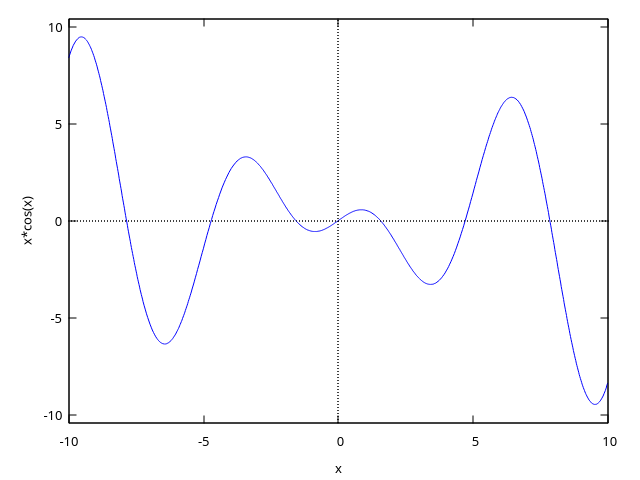
\includegraphics[scale=0.7]{images/2022-03-21_plot_1.png}
\end{figure}

In a similar spirit we can also evaluate $\int x e^x dx$. We consider

\bee
I(a) = \int e^{ax} dx = \frac{1}{a} e^{ax}
\eee

Differentiating wrt $a$ yields

\bee
\frac{dI(a)}{da} = \int \left( \frac{d}{da} e^{ax} \right) dx = \int x e^{ax} dx
\eee

Taking the derivative from the result of $I(a)$ yields

\bee
\frac{d}{da} \left( \frac{1}{a} e^{ax} \right) = \frac{xe^{ax}a - e^{ax}}{a^2}
\eee

and we obtain

\bee
\boxed{
    \int x e^{ax} dx = \frac{(xa - 1) e^{ax}}{a^2}
}
\eee

The integrand $x e^{ax}$ (for different values of $a$) is shown in the following Figure.

\begin{figure}[H]
    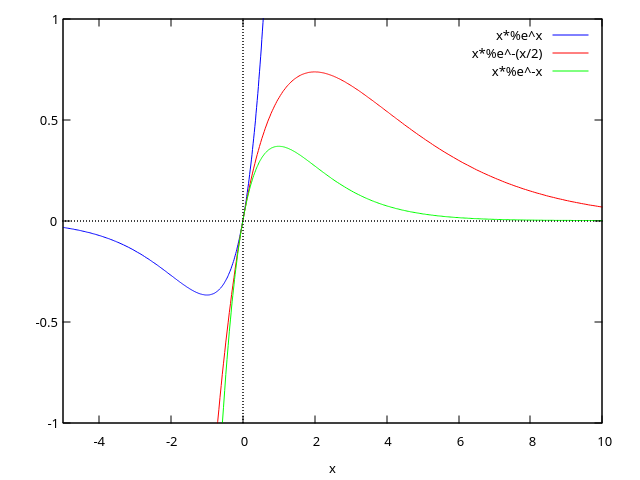
\includegraphics[scale=0.7]{images/2022-03-21_plot_2.png}
\end{figure}
    

\subsection{Integrating the Normal Distribution}

Now, let's use the machinery in earnest and try the following integral,

\bee
I = \int_{- \infty}^\infty e^{-\frac{x^2}{2}} dx
\eee

We consider the integral over the right interval and introduce

\bee
g(t) = \left( \int_{0}^t e^{-\frac{x^2}{2}} dx \right)^2
\eee

Our original integral then becomes

\bee
I = \int_{- \infty}^\infty e^{-\frac{x^2}{2}} dx = 2 \sqrt{g(\infty)}
\eee

Let's apply \eqref{2022-03-21:eq1} to calculate $dg/dt$ (note that the only thing that varies is the upper limit and we therefore have only the $f(b, \alpha) \frac{db}{d \alpha}$ term),

\bee
\frac{dg}{dt} = 2 \left( \int_{0}^t e^{-\frac{x^2}{2}} dx \right) \frac{d}{dt} \left( \int_{0}^t e^{-\frac{x^2}{2}} dx \right)
= 2 \left( \int_{0}^t e^{-\frac{x^2}{2}} dx \right) e^{-\frac{t^2}{2}} = 2 \int_{0}^t e^{-\frac{x^2 + t^2}{2}} dx
\eee

Next we make a variable substitution $y = x/t \rightarrow x = yt \rightarrow dx = t dy$ and arrive at

\bee
\frac{dg}{dt} = 2 \int_{0}^1 t e^{-\frac{y^2 t^2 + t^2}{2}} dy = 2 \int_{0}^1 t e^{-\frac{t^2 (1 + y^2)}{2}} dy
\eee

The whole purpose of the substitution is that we can express the integrand as derivative as follows,

\bee
2 t e^{-\frac{t^2 (1 + y^2)}{2}} = \frac{\partial}{\partial t} \left( - \frac{2 e^{-\frac{t^2 (1 + y^2)}{2}} }{1+y^2} \right)
\eee

and therefore

\bee
\frac{dg}{dt} = \int_{0}^1 \frac{\partial}{\partial t} \left( \frac{2 e^{-\frac{t^2 (1 + y^2)}{2}} }{1+y^2} \right) = -2 \frac{d}{dt} \int_{0}^1 \frac{e^{-\frac{t^2 (1 + y^2)}{2}} }{1+y^2} dy
\eee

We can integrate this expression with respect to $t$ and obtain

\be\label{2022-03-21:eq2}
g(t) = -2 \int_{0}^1 \frac{e^{-\frac{t^2 (1 + y^2)}{2}} }{1+y^2} dy + C
\ee

where $C$ is the (important) integration constant. In the definition of $g(t)$ we set $t=0$ and then

\bee
g(0) = \left( \int_{0}^t e^{-\frac{x^2}{2}} dx \right)^2 = 0
\eee

Now we set $t = 0$ in $\int_{0}^1 \frac{e^{-\frac{t^2 (1 + y^2)}{2}} }{1+y^2} dy$ which yields $\int_{0}^1 \frac{1}{1+y^2} dy = \left. \arctan y \right|_0^1 = \frac{\pi}{4}$. We can combine things at $t=0$ and obtain

\bee
g(0) = 0 = -2 \frac{\pi}{4} + C \rightarrow C = \frac{\pi}{2}
\eee

and so

\bee
g(t) = -2 \int_{0}^1 \frac{e^{-\frac{t^2 (1 + y^2)}{2}} }{1+y^2} dy + \frac{\pi}{2}
\eee

We are interested in $I = 2 \sqrt{g(\infty)}$, therefore

\bee
g(\infty) = -2 \lim_{t \rightarrow \infty} \int_{0}^1 \frac{e^{-\frac{t^2 (1 + y^2)}{2}} }{1+y^2} dy + \frac{\pi}{2}
\eee

For increasing $t$, the integrals gets "peakier" and in the limit becomes zero; therefore $g(\infty) = \frac{\pi}{2}$, from which follows

\bee
\sqrt{g(\infty)} = \sqrt{\frac{\pi}{2}} \rightarrow I = 2 \sqrt{g(\infty)} = 2 \sqrt{\frac{\pi}{2}} = \sqrt{2 \pi}
\eee

and we arrive at

\bee
\boxed{
I = \int_{- \infty}^\infty e^{-\frac{x^2}{2}} dx = \sqrt{2 \pi}}
\eee

The integrand is symmetric, therefore we have

\bee
\int_{0}^\infty e^{-\frac{x^2}{2}} dx = \sqrt{\frac{\pi}{2}}
\eee

We can use this result to calculate another (even scarier looking) integral. Let's substitute $u = x / \sqrt{2}$ and obtain ($du/dx = 1 / \sqrt{2} \rightarrow dx = \sqrt{2} du$)

\bee
\int_{0}^\infty e^{- u^2 } \sqrt{2} du = \sqrt{\frac{\pi}{2}}
\eee

and therefore

\bee
\boxed{
    \int_{0}^\infty e^{- u^2 } du = \frac{\sqrt{\pi}}{2}
}
\eee

Now we substitute $t = e^{-u^2}$ from which follows $u = \sqrt{- \log t}$ and $dt/du = -2ue^{-u^2} = -2ut$. The integration limits transform according to $u = 0 \rightarrow t = 1$ and $u = \infty \rightarrow t = 0$ and the integral becomes

\bee
\int_{0}^\infty e^{- u^2 } du = - \int_1^0 t \frac{dt}{2ut} = \int_0^1 \frac{dt}{2u} = \int_0^1 \frac{dt}{2 \sqrt{- \log t} }
\eee

We therefore have

\bee
\int_0^1 \frac{dt}{2 \sqrt{- \log t} } = \frac{\sqrt{\pi}}{2} \rightarrow \int_0^1 \frac{dt}{\sqrt{- \log t} } = \sqrt{\pi}
\eee

To summarize, we calculated

\bee
\boxed{
    \int_0^1 \frac{dt}{\sqrt{- \log t} } = \sqrt{\pi}
}
\eee

The following Figure shows the integrand.

\begin{figure}[H]
    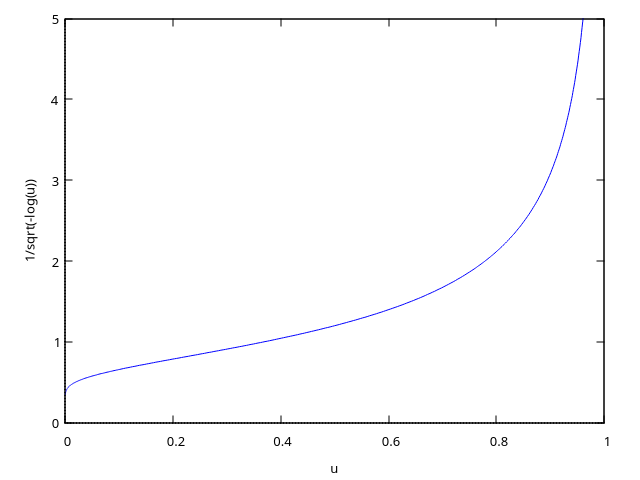
\includegraphics[scale=0.7]{images/2022-03-21_plot_2a.png}
\end{figure}

\subsection{Integrating Cosine $\times$ Normal Distribution}

We consider the integral

\bee
I(t) = \int_0^\infty \cos(tx) e^{-x^2/2} dx
\eee

For $t=0$ this becomes $\sqrt{\frac{\pi}{2}}$ (using the previous result). Anyway, let's differentiate wrt $t$ and we obtain

\bee
\frac{d}{dt} I(t) = \int_0^\infty -x \sin(tx) e^{-x^2/2} dx
\eee

Interestingly, this can be solved via integration by parts. We set $u = \sin(tx)$ and $v' = -x e^{-x^2/2}$. Then $u' = t \cos(tx)$ and $v = e^{-x^2/2}$ (via the substitution $u = -x^2 / 2$). Integrating by parts yields

\begin{align*}
    \int_0^\infty -x \sin(tx) e^{-x^2/2} dx &= - \left. \frac{x^2}{2} e^{-x^2/2} \right|_0^\infty - \int_0^\infty t \cos(tx) e^{-x^2/2} dx \\ &= 0 - \int_0^\infty t \cos(tx) e^{-x^2/2} dx \\ &= - t I(t)
\end{align*}

So we have the following ODE

\bee
\frac{d}{dt} I(t) = - t I(t) \rightarrow \frac{dI(t)}{I(t)} = - t dt
\eee

and we can integrate both sides to obtain

\bee
\log I(t) = - \frac{t^2}{2} + C
\eee

Using the fact that we know $I(0) = \sqrt{\frac{\pi}{2}}$ we can determine the constant of integration $C$ as $\log I(0) = C \rightarrow C = \log(\sqrt{ \frac{\pi}{2} })$ and therefore

\bee
\log I(t) = - \frac{t^2}{2} + \log\left( \sqrt{ \frac{\pi}{2} } \right)
\eee

from which we obtain

\bee
\boxed{
    I(t) = \int_0^\infty \cos(tx) e^{-x^2/2} dx = \sqrt{ \frac{\pi}{2} } e^{- \frac{t^2}{2}}
}
\eee

The integrand $\cos(tx) e^{-x^2/2}$ is shown for different values of $t$ in the following Figure. The larger $t$, the more the function oscillates and the more positive and negative areas cancel each other, and therefore, the smaller the integral becomes.

\begin{figure}[H]
    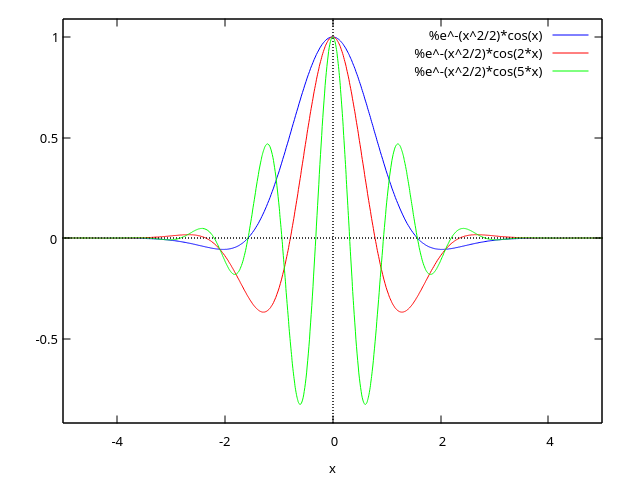
\includegraphics[scale=0.7]{images/2022-03-21_plot_3.png}
\end{figure}

As the integrand is an even function, we have

\bee
\int_{-\infty}^\infty \cos(tx) e^{-x^2/2} dx = \sqrt{ 2\pi } e^{- \frac{t^2}{2}}
\eee

Next we sneak in a cosine expression and use $\cos(s + tx) = \cos(s) \cos(tx) - \sin(s)\sin(tx)$

\begin{equation}
    \int_{-\infty}^\infty \cos(s + tx) e^{-x^2/2} dx = \int_{-\infty}^\infty \cos(s) \cos(tx) e^{-x^2/2} dx - \int_{-\infty}^\infty \sin(s) \sin(tx) e^{-x^2/2} dx
\end{equation}

The second integrand is an odd function and therefore the integral vanishes; so we have

\begin{equation}
    \int_{-\infty}^\infty \cos(s + tx) e^{-x^2/2} dx = \int_{-\infty}^\infty \cos(s) \cos(tx) e^{-x^2/2} dx = \cos(s) \int_{-\infty}^\infty \cos(tx) e^{-x^2/2} dx
\end{equation}

and finally

\begin{equation}
    \boxed{
    \int_{-\infty}^\infty \cos(s + tx) e^{-x^2/2} dx = \sqrt{ 2\pi } \cos(s) e^{- \frac{t^2}{2}}
    }
\end{equation}

The following Figure shows the integrand for different values of $s$. For increasing values of $s$, the oscillations inside the $e^{-x^2/2}$ envelope shift to the left and the larger the negative area gets, causing the integral to become smaller (and negative, eventually; e.g. $\cos(4) \approx -0.6536$).

\begin{figure}[H]
    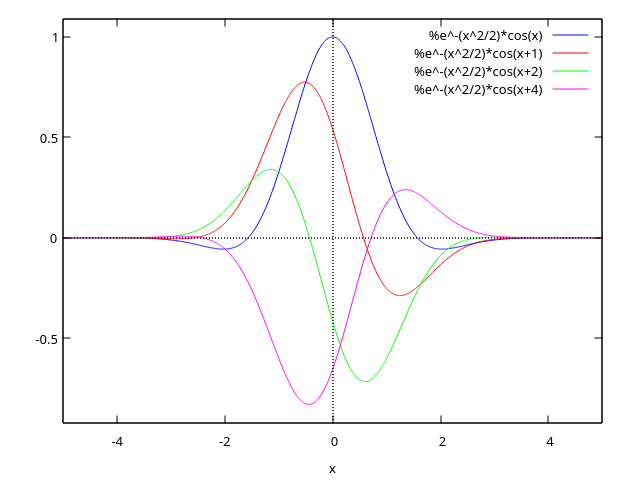
\includegraphics[scale=0.7]{images/2022-03-21_plot_4.png}
\end{figure}

\subsection{One Last - $\cos / (x^2+b^2)$}

Let's consider one last integral where we solve an ODE to actually solve an integral,

\bee
I(a) = \int_0^\infty \frac{\cos ax}{x^2 + b^2} dx
\eee

We first integrate by parts and set $u = 1/(x^2+b^2), v' = \cos ax$ to get

\bee
\frac{du}{dx} = - \frac{2x}{(x^2+b^2)^2}, v = \frac{\sin ax}{a}
\eee

Therefore, we have

\bee
I(a) = \left. \frac{\sin ax}{a (x^2+b^2)^2} \right|_0^\infty + \frac{2}{a} \int_0^\infty \frac{x \sin ax}{(x^2 + b^2)^2} dx
\eee

The first term vanishes and we arrive at

\be\label{2022-03-21:eq3}
I(a) = \frac{2}{a} \int_0^\infty \frac{x \sin ax}{(x^2 + b^2)^2} dx
\ee

Multiply with $a$ and differentiate wrt $a$ to obtain

\bee
a \frac{dI(a)}{da} + I(a) = 2 \int_0^\infty \frac{x^2 \cos ax}{(x^2 + b^2)^2} dx
\eee

We can make a partial fraction expansion of the integrand and obtain

\bee
\frac{x^2 \cos ax}{(x^2 + b^2)^2} = \frac{\cos ax}{(x^2 + b^2)} - \frac{b^2 \cos ax}{(x^2 + b^2)^2}
\eee

Therefore, our integral becomes

\bee
2 \int_0^\infty \frac{x^2 \cos ax}{(x^2 + b^2)^2} dx = 2 \int_0^\infty \frac{\cos ax}{(x^2 + b^2)} dx - 2b^2 \int_0^\infty \frac{\cos ax}{(x^2 + b^2)^2} dx
\eee

The first integral happens to be $I(a)$ and we obtain

\bee
a \frac{dI(a)}{da} + I(a) = 2I(a) - 2b^2 \int_0^\infty \frac{\cos ax}{(x^2 + b^2)^2} dx \rightarrow a \frac{dI(a)}{da} - I(a) = - 2b^2 \int_0^\infty \frac{\cos ax}{(x^2 + b^2)^2} dx
\eee

Let's differentiate again wrt $a$ to obtain

\bee
a \frac{d^2I(a)}{da^2} + \frac{dI(a)}{da} - \frac{dI(a)}{da} = - 2b^2 \int_0^\infty \frac{x \sin ax}{(x^2 + b^2)^2} dx
\eee

or

\bee
a \frac{d^2I(a)}{da^2} = - 2b^2 \int_0^\infty \frac{x \sin ax}{(x^2 + b^2)^2} dx
\eee

Luckily, the integral has already appeared in \eqref{2022-03-21:eq3} and so we have

\bee
a \frac{d^2I(a)}{da^2} = 2b^2 \frac{a}{2} I(a) \rightarrow \frac{d^2I(a)}{da^2} - b^2 I(a) = 0
\eee

whcih is a second order ODE for the unknown function (which is actually our integral solution!) $I(a)$. An Ansatz is $I(a) = C e^{ka}$ (with $C$ and $k$ constants) and inserting this yields

\bee
I(a) = C_1 e^{ab} + C_2 e^{-ab}
\eee

All that is left is to calculate the constants $C_1$ and $C_2$. From the integal definition we see that

\bee
I(0) = \int_0^\infty \frac{1}{x^2 + b^2} dx = \frac{1}{b} \left. \arctan \frac{a}{b} \right|_0^\infty = \frac{\pi}{2b}
\eee

From \eqref{2022-03-21:eq3} we can obtain an expression for $I(\infty)$ as

\bee
I(\infty) = \lim_{a \rightarrow \infty} \frac{2}{a} \int_0^\infty \frac{x \sin ax}{(x^2 + b^2)^2} dx = 0
\eee

and we can use these two values to calculate $C_1$ and $C_2$.

\begin{align*}
    I(\infty) &= 0 \rightarrow C_1 = 0 \\
    I(0) &= \frac{\pi}{2b} = C_1 + C_2 \rightarrow C_2 = \frac{\pi}{2b}
\end{align*}

Therefore, our solution finally is

\bee
\boxed{
    I(a) = \int_0^\infty \frac{\cos ax}{x^2 + b^2} dx = \frac{\pi}{2b} e^{-ab}
}
\eee

The integrand is shown in the following Figure for different values of $a$ and $b$. Larger values of $a$ cause faster oscillations and therefore a larger contribution of the negative part. Increasing $b$ decreases the amplitude, resulting in less area as well.

\begin{figure}[H]
    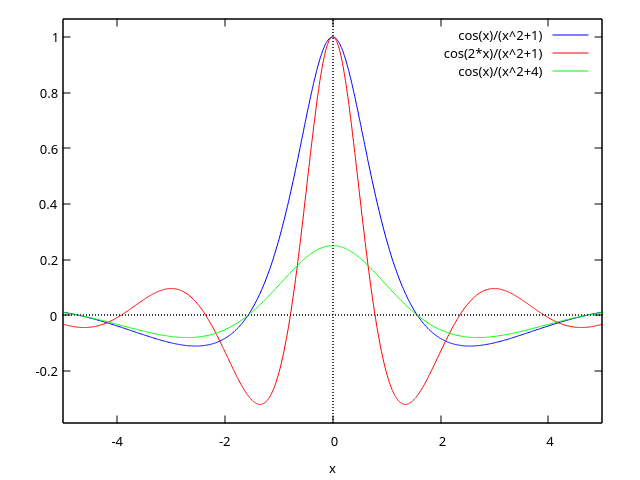
\includegraphics[scale=0.7]{images/2022-03-21_plot_5.png}
\end{figure}



%%% Local Variables:
%%% mode: latex
%%% TeX-master: "journal"
%%% End:
